\usetikzlibrary{calc}

\def\layersep{2.5cm}

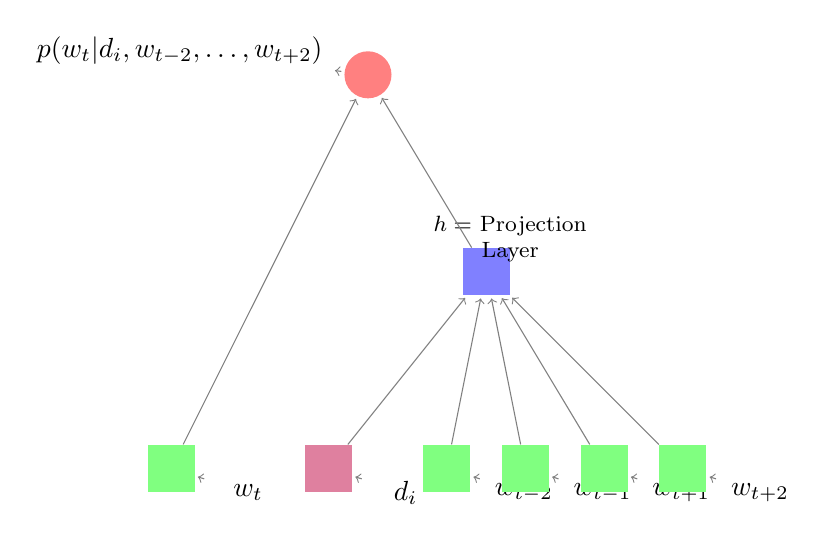
\begin{tikzpicture}[shorten >=1pt,->,draw=black!50, node distance=\layersep,transform shape,rotate=90]  %<-- rotate the NN
    \tikzstyle{every pin edge}=[<-,shorten <=1pt]
    \tikzstyle{neuronrect}=[rectangle,fill=black!25, minimum size=17pt, inner sep=0pt] %
    \tikzstyle{neuroncircle}=[circle,fill=black!25,minimum size=17pt,inner sep=0pt]
    \tikzstyle{input neuron}=[neuronrect, fill=green!50];
    \tikzstyle{doc neuron}=[neuronrect, fill=purple!50];
    \tikzstyle{output neuron}=[neuroncircle, fill=red!50];
    \tikzstyle{hidden neuron}=[neuronrect, fill=blue!50];
    \tikzstyle{annot} = [text width=4em, text centered]
    \tikzset{hoz/.style={rotate=-90}}   %<--- for labels
    % Draw the input layer nodes
    %\foreach \name / \y in {1,...,4}
    % This is the same as writing \foreach \name / \y in {1/1,2/2,3/3,4/4}
        %\node[input neuron, pin=left:\rotatebox{-90}{\parbox[t][][r]{8mm}{\centering $w_{t-j}$}}] (I-\name) at (0,-\y) {};

	\node[input neuron, pin=left:\rotatebox{-90}{\parbox[t][][r]{8mm}{\centering $w_{t}$}}] (W-0) at (0,2.5) {};    

    \node[doc neuron, pin=left:\rotatebox{-90}{\parbox[t][][r]{8mm}{\centering $d_{i}$}}] (I-0) at (0,0.5) {};    

    \node[input neuron, pin=left:\rotatebox{-90}{\parbox[t][][r]{8mm}{\centering $w_{t-2}$}}] (I-1) at (0,-1) {};
    \node[input neuron, pin=left:\rotatebox{-90}{\parbox[t][][r]{8mm}{\centering $w_{t-1}$}}] (I-2) at (0,-2) {};
    \node[input neuron, pin=left:\rotatebox{-90}{\parbox[t][][r]{8mm}{\centering $w_{t+1}$}}] (I-3) at (0,-3) {};
    \node[input neuron, pin=left:\rotatebox{-90}{\parbox[t][][r]{8mm}{\centering $w_{t+2}$}}] (I-4) at (0,-4) {};    

    % Draw the hidden layer nodes
    % \foreach \name / \y in {1,...,5}
        \path[yshift=0.5cm]
        node[hidden neuron] (H-1) at (\layersep,-2.0 cm) [label=below:\rotatebox{-90}{\parbox[t][][r]{20mm}{\centering \footnotesize $h=$ Projection Layer}}] {};

    % Draw the output layer node
    \node[output neuron, pin={[pin edge={->}]right:\rotatebox{-90}{$p(w_{t}|d_{i}, w_{t-2}, \ldots, w_{t+2})$}}] (O) at (\layersep + \layersep,0) {};
    %\node[output neuron,pin={[pin edge={->}]right:\rotatebox{-90}{$p(w_{t}|d_{i}, w_{t-2}, \ldots, w_{t+2})$}}, right of=H-1] (O) {};

    % Connect word vectors to projection later
    \foreach \source in {1,...,4}
        \path (I-\source) edge (H-1);

    %Connect Middle Word to Output Node
	\path (W-0) edge (O);            

	%Connect Doc Embedding to Projection Layer
	\path (I-0) edge (H-1);            

    %Connect Projection Layer to Output
    \path (H-1) edge (O);

    % Annotate the layers
    % \node[annot,above of=H-1, node distance=1cm,hoz] (hl) {Hidden layer};
    % \node[annot,left of=hl,hoz] {Input layer};
    % \node[annot,right of=hl,hoz] {Output layer};
\end{tikzpicture}

% \begin{tikzpicture}[scale=1.0, transform shape]
% % Macros
% % relative positioning
% \newcommand{\at}[3]{
%   \begin{scope}[shift={(#1,#2)}]
%     #3
%   \end{scope} 
% }

% % Embeddings
% \newcommand{\embcolor}{PineGreen}
% \newcommand{\ye}{1}
% \newcommand{\he}{1.5}
% \newcommand{\we}{1}
% \newcommand{\gape}{1}

% \newcommand{\xc}{0.5}
% \newcommand{\xa}{\xc+\we+\gape}
% \newcommand{\xb}{\xa+\we+\gape}
% \newcommand{\xu}{\xb+\we+\gape}
% \newcommand{\xw}{\xu+\we+\gape}

% \draw [thick]
% 	(\xb+\we/2,\ye+\he+0.5) node[above,\embcolor] {Entities, $\mathcal{E}$};
% % Draw curly braces using path decoration
% \draw [\embcolor,decorate,decoration={brace,amplitude=5pt},xshift=-15pt] %,yshift=-9pt] 
% 	(\xc,\ye)  -- (\xc,\ye+\he) node [align=right,left,\embcolor,midway,xshift=-5pt]
% 	{Model Parameters, $\Phi$\\{\small $k$-dimensional entity vectors}};
% % Users
% \draw[<->,\embcolor!50]
% 	(\xu,\ye-0.15) -- (\xu+\we,\ye-0.15) 
% 	node[pos=.5,shape=rectangle,fill=white,draw=none] {\scriptsize $k$};
% \draw[<->,\embcolor!50] 
% 	(\xu+\we+0.3,\ye) -- (\xu+\we+0.3,\ye+\he) 
% 	node[pos=.5,shape=rectangle,fill=white,draw=none] {\scriptsize $|U|$};
% \draw [semithick,fill=gray!10] 
% 	(\xu,\ye) rectangle (\xu+\we,\ye+\he)
% 	(\xu+\we/2.0,\ye+\he/2.0) node[draw=none,shape=circle] (nodeU) {$\Phi_U$}
% 	(\xu+\we/2.0,\ye+\he) node[above] {\scriptsize Users, U};
% % Businesses
% \draw[<->,\embcolor!50]
% 	(\xb,\ye-0.15) -- (\xb+\we,\ye-0.15) 
% 	node[pos=.5,shape=rectangle,fill=white,draw=none] {\scriptsize $k$};
% \draw[<->,\embcolor!50] 
% 	(\xb+\we+0.3,\ye) -- (\xb+\we+0.3,\ye+\he) 
% 	node[pos=.5,shape=rectangle,fill=white,draw=none] {\scriptsize $|B|$};
% \draw [semithick,fill=gray!10] 
% 	(\xb,\ye) rectangle (\xb+\we,\ye+\he)
% 	(\xb+\we/2.0,\ye+\he/2.0) node[draw=none,shape=circle] (nodeB) {$\Phi_B$}
% 	(\xb+\we/2.0,\ye+\he) node[above] {\scriptsize Businesses, B};
% % Categories
% \draw[<->,\embcolor!50]
% 	(\xc,\ye-0.15) -- (\xc+\we,\ye-0.15) 
% 	node[pos=.5,shape=rectangle,fill=white,draw=none] {\scriptsize $k$};
% \draw[<->,\embcolor!50] 
% 	(\xc+\we+0.3,\ye) -- (\xc+\we+0.3,\ye+\he) 
% 	node[pos=.5,shape=rectangle,fill=white,draw=none] {\scriptsize $|C|$};
% \draw [semithick,fill=gray!10] 
% 	(\xc,\ye) rectangle (\xc+\we,\ye+\he)
% 	(\xc+\we/2.0,\ye+\he/2.0) node[draw=none,shape=circle] (nodeC) {$\Phi_C$}
% 	(\xc+\we/2.0,\ye+\he) node[above] {\scriptsize Categories, C};
% % Attributes
% \draw[<->,\embcolor!50]
% 	(\xa,\ye-0.15) -- (\xa+\we,\ye-0.15) 
% 	node[pos=.5,shape=rectangle,fill=white,draw=none] {\scriptsize $k$};
% \draw[<->,\embcolor!50] 
% 	(\xa+\we+0.3,\ye) -- (\xa+\we+0.3,\ye+\he) 
% 	node[pos=.5,shape=rectangle,fill=white,draw=none] {\scriptsize $|A|$};
% \draw [semithick,fill=gray!10] 
% 	(\xa,\ye) rectangle (\xa+\we,\ye+\he)
% 	(\xa+\we/2.0,\ye+\he/2.0) node[draw=none,shape=circle] (nodeA) {$\Phi_A$}
% 	(\xa+\we/2.0,\ye+\he) node[above] {\scriptsize Attributes, A};
% % Words
% \draw[<->,\embcolor!50]
% 	(\xw,\ye-0.15) -- (\xw+\we,\ye-0.15) 
% 	node[pos=.5,shape=rectangle,fill=white,draw=none] {\scriptsize $k$};
% \draw[<->,\embcolor!50] 
% 	(\xw+\we+0.3,\ye) -- (\xw+\we+0.3,\ye+\he) 
% 	node[pos=.5,shape=rectangle,fill=white,draw=none] {\scriptsize $|W|$};
% \draw [semithick,fill=gray!10] 
% 	(\xw,\ye) rectangle (\xw+\we,\ye+\he)
% 	(\xw+\we/2.0,\ye+\he/2.0) node[draw=none,shape=circle] (nodeW) {$\Phi_W$}
% 	(\xw+\we/2.0,\ye+\he) node[above] {\scriptsize Review words, W};

% % Matrices (Relations)
% \newcommand{\relcolor}{RoyalBlue}
% \newcommand{\ym}{-2}
% \newcommand{\hm}{2}
% \newcommand{\wm}{2}
% \newcommand{\gapm}{0.75}
% \newcommand{\gridmcolor}{gray!10}

% \newcommand{\xCB}{-2}
% \newcommand{\xAB}{\xCB+\wm+\gapm}
% \newcommand{\xR}{\xAB+\wm+\gapm}
% \newcommand{\xBW}{\xR+\wm+\gapm}
% \newcommand{\xUW}{\xBW+\wm+\gapm}

% \newcommand{\sparsegrid}{
% 	\draw [step=0.1,thin,\gridmcolor] (0,0) grid (\wm,\hm);
% 	\foreach \i in {0,1,...,75}{
% 		\pgfmathsetmacro{\xcell}{int(rnd*20)*\wm/20}
% 		\pgfmathsetmacro{\ycell}{int(rnd*20)*\wm/20}
% 		\fill[gray!20] (\xcell,\ycell) rectangle (\xcell+0.1,\ycell+0.1);
% 	}
% }

% \draw [thick]
% 	(\xR+\wm/2,\ym-0.5) node[below,\relcolor] {Relations, $\mathcal{R}$};
% % Draw curly braces using path decoration
% \draw [\relcolor,decorate,decoration={brace,amplitude=5pt},xshift=-15pt] %,yshift=-9pt] 
% 	(\xCB,\ym)  -- (\xCB,\ym+\hm) node [align=right,left,\relcolor,midway,xshift=-5pt]
% 	{Partial Observations\\{\small Predict missing data}};

% % CB
% \draw[<->,\relcolor!50]
% 	(\xCB,\ym+\hm+0.15) -- (\xCB+\wm,\ym+\hm+0.15) 
% 	node[pos=.5,shape=rectangle,fill=white,draw=none] {\scriptsize $|C|$};
% \draw[<->,\relcolor!50] 
% 	(\xCB+\wm+0.3,\ym) -- (\xCB+\wm+0.3,\ym+\hm) 
% 	node[pos=.5,shape=rectangle,fill=white,draw=none] {\scriptsize $|B|$};
% \at{\xCB}{\ym}{\sparsegrid}
% \draw [thick] 
% 	(\xCB,\ym) rectangle (\xCB+\wm,\ym+\hm)
% 	(\xCB+\wm/2.0,\ym+\hm/2.0) node[draw=none,shape=circle] (nodeCB) {C}
% 	(\xCB+\wm/2.0,\ym) node[below] {\scriptsize Business Categories};
% % AB
% \draw[<->,\relcolor!50]
% 	(\xAB,\ym+\hm+0.15) -- (\xAB+\wm,\ym+\hm+0.15) 
% 	node[pos=.5,shape=rectangle,fill=white,draw=none] {\scriptsize $|A|$};
% \draw[<->,\relcolor!50] 
% 	(\xAB+\wm+0.3,\ym) -- (\xAB+\wm+0.3,\ym+\hm) 
% 	node[pos=.5,shape=rectangle,fill=white,draw=none] {\scriptsize $|B|$};
% \at{\xAB}{\ym}{\sparsegrid}
% \draw [thick] 
% 	(\xAB,\ym) rectangle (\xAB+\wm,\ym+\hm)
% 	(\xAB+\wm/2.0,\ym+\hm/2.0) node[draw=none,shape=circle] (nodeAB) {A}
% 	(\xAB+\wm/2.0,\ym) node[below] {\scriptsize Business Attributes};
% % R
% \draw[<->,\relcolor!50]
% 	(\xR,\ym+\hm+0.15) -- (\xR+\wm,\ym+\hm+0.15) 
% 	node[pos=.5,shape=rectangle,fill=white,draw=none] {\scriptsize $|U|$};
% \draw[<->,\relcolor!50] 
% 	(\xR+\wm+0.3,\ym) -- (\xR+\wm+0.3,\ym+\hm) 
% 	node[pos=.5,shape=rectangle,fill=white,draw=none] {\scriptsize $|B|$};
% \at{\xR}{\ym}{\sparsegrid}
% \draw [thick] 
% 	(\xR,\ym) rectangle (\xR+\wm,\ym+\hm)
% 	(\xR+\wm/2.0,\ym+\hm/2.0) node[draw=none,shape=circle] (nodeR) {R}
% 	(\xR+\wm/2.0,\ym) node[below] {\scriptsize User/Business Ratings};
% % BW
% \draw[<->,\relcolor!50]
% 	(\xBW,\ym+\hm+0.15) -- (\xBW+\wm,\ym+\hm+0.15) 
% 	node[pos=.5,shape=rectangle,fill=white,draw=none] {\scriptsize $|W|$};
% \draw[<->,\relcolor!50] 
% 	(\xBW+\wm+0.3,\ym) -- (\xBW+\wm+0.3,\ym+\hm) 
% 	node[pos=.5,shape=rectangle,fill=white,draw=none] {\scriptsize $|B|$};
% \at{\xBW}{\ym}{\sparsegrid}
% \draw [thick] 
% 	(\xBW,\ym) rectangle (\xBW+\wm,\ym+\hm)
% 	(\xBW+\wm/2.0,\ym+\hm/2.0) node[draw=none,shape=circle] (nodeBW) {BW}
% 	(\xBW+\wm/2.0,\ym) node[below] {\scriptsize Reviews for Business};
% % UW
% \draw[<->,\relcolor!50]
% 	(\xUW,\ym+\hm+0.15) -- (\xUW+\wm,\ym+\hm+0.15) 
% 	node[pos=.5,shape=rectangle,fill=white,draw=none] {\scriptsize $|W|$};
% \draw[<->,\relcolor!50] 
% 	(\xUW+\wm+0.3,\ym) -- (\xUW+\wm+0.3,\ym+\hm) 
% 	node[pos=.5,shape=rectangle,fill=white,draw=none] {\scriptsize $|U|$};
% \at{\xUW}{\ym}{\sparsegrid}
% \draw [thick] 
% 	(\xUW,\ym) rectangle (\xUW+\wm,\ym+\hm)
% 	(\xUW+\wm/2.0,\ym+\hm/2.0) node[draw=none,shape=circle] (nodeUW) {UW}
% 	(\xUW+\wm/2.0,\ym) node[below] {\scriptsize Reviews by Users};

% % Edges between embeddings and matrices
% \newcommand{\arrowcolor}{black}
% \draw[\arrowcolor,->] (nodeC) -- (nodeCB);
% \draw[\arrowcolor,->] (nodeB) -- (nodeCB);

% \draw[\arrowcolor,->] (nodeA) -- (nodeAB);
% \draw[\arrowcolor,->] (nodeB) -- (nodeAB);

% \draw[\arrowcolor,->] (nodeU) -- (nodeR);
% \draw[\arrowcolor,->] (nodeB) -- (nodeR);

% \draw[\arrowcolor,->] (nodeW) -- (nodeBW);
% \draw[\arrowcolor,->] (nodeB) -- (nodeBW);

% \draw[\arrowcolor,->] (nodeU) -- (nodeUW);
% \draw[\arrowcolor,->] (nodeW) -- (nodeUW);
% \end{tikzpicture}